\documentclass[11pt, twocolumn]{article}

\usepackage{amsmath}
\usepackage{amssymb}
\usepackage{graphicx}
\usepackage{booktabs}
\usepackage{fancyvrb}

\begin{document}
\title{The Effectiveness of Brightness Metrics for Ball Detection}
\author{Marcus Christiansen, Will Gantt}
\maketitle

\abstract{\textbf{Broadly, the goal of this project was to determine whether brightness measurements could be an effective tool for ball detection. Specifically, we considered how such metrics might be incorporated into the spot filter; first, in the identification of blacks spots, second, in a comparison between the brightness values of the top and bottom hemispheres of the ball itself, and, third, in a comparison between the brightness values of the regions immediately above and below the ball. Regarding black spots, we found that there is little difference in brightness between true and false positive instances. In the comparison of hemispheres, we found that \ldots. In the comparison of above-ball and below-ball regions, we saw \ldots.}}
\section{Overview}
Since the RoboCup League's recent decision to replace the traditional orange ball with one more reminiscent of a classical soccer ball, teams have been faced with a slew of new vision challenges. As the ball's primary color is now white, teams must find novel ways to distinguish it from other white objects, including field lines, goal posts, and robots. Furthermore, they must differentiate the black pentagons of the ball from chimeras such as robot joints and other dark spots on the field. Thus, color alone can no longer serve as a reliable marker. Consequently, the Northern Bites have implemented a variety of additional checks. These include a determination of the expected radius of the ball at different locations on the field, an evaluation of the spatial relationships between black spots, and more obvious checks to verify that a candidate ball is in fact on the field. \\
\indent Although the ball detector concerns itself to a great extent with white and black, it makes almost no use of brightness inputs. Since black is notoriously difficult to characterize strictly on the basis of color (U and V) values, we wished to see whether brightness (the Y image) could provide some helpful information in this regard. 
\section{Experiment}
Currently, robots identify candidate balls using a spot filter. The basic principle consists in scanning an image with a ``filter,'' which comprises a small, square-shaped region nested within a larger one. At each position in the scan, the filter performs a simple check to determine whether the outer region is whiter on average than the inner one. The idea is that a ball will tend to be darker in the middle, since the black spots typically fall closer to its center, and whiter around the edges. [Include a graphic?] \\
\indent The tests we ran operated on spots that the detector already identified. That is, the tests were intended to filter, rather than discover, candidate balls. The first test considered the median Y-value of each detected black spot, with the goal of determining whether there was any consistent, significant difference between true positives (black spots actually on the ball) and false positives. The second compared the median Y-values of the top and bottom halves of the inner region of a white spot (a candidate ball). We reasoned that, because the field is lit from above, the top half of a ball should tend to be brighter than the bottom half. By the same logic, we hypothesized that the shadow cast by the ball on the field itself should mean that the area of the field directly below the ball will be darker than the area directly above it. This was implemented as a third test. \\
\indent All three tests were conducted on the same data, which comprised sets of logs taken in the robotics lab at levels of illumination of 150, 300, and 450 lux.\footnote{In truth, measuring the brightness of an entire room with this level of accuracy is impossible, given imperfections in the light meter, as well as minor fluctuations in the illumination of the room itself. These values should therefore be taken as approximate.} For each level of brightness, we placed the robot in 12 different scenarios, and for each scenario, we made adjustments to some combination of the following variables:
\begin{itemize}
\item The presence of the ball on the field (i.e., \emph{whether} the ball is on the field)
\item The robot's distance from the ball.
\item The ball's position on the field.
\item The robot's position on the field.
\item The number of other robots present on the field.
\end{itemize}
\subsection{Black Spot Detection}
In the first test, we differentiated true and false positive black spots ourselves by looking at the output of the ``DebugImageView'' module in the tool, which circles in yellow all of the black spots that the ball detector has identified. For each log, we documented the total number of black spots detected, the number of true positives, the number of false positives, the Y values of each spot, the number of other robots on the field, and the presence of the ball on the field (i.e. whether it was in the image or not). Once we had obtained this information for all logs at a given illumination level, we calculated the median, mean, and standard deviation of the true and false positives.
\subsection{Hemisphere Comparison}
\subsection{Region Above and Below Ball}
\section{Algorithm}
As our goal in this project was merely to see whether brightness tests could be used effectively in the ball detector, and not to write game-ready ball detection code, we were not especially concerned with algorithmic efficiency. Nonetheless, we have included the functions we wrote at the end of this paper. What follows are high-level descriptions of what each does.
\begin{description}
\item[\texttt{getMedianBrightness}:] As mentioned in section 2, a spot consists of a smaller square region nested within a larger one. This function determines the median Y value of the inner region of a black spot by simply iterating over all of the pixels in that region, and adding the Y value of each to a vector. The vector is then sorted and the element at the median index is returned.
\item[\texttt{topOfBallBrighterThanBottom}:] Takes the inner region of a ball (a white spot) and divides it into a top half and a bottom half. The median Y values of each half are determined using the same method as in \texttt{getMedianBrightness}, and both are returned together as a pair of doubles.
\item[\texttt{aboveBallBrighterThanBelowBall}:] This uses the same basic approach as the previous function but considers the rectangular areas (1) between the top edge of the white spot and the top edge of the inner region, and (2) between the bottom edge of the white spot and the bottom edge of the inner region. Both of these areas cover some of the ball, as well as some of the field. The function determines the median Y values of each region and returns them as a pair of  doubles. 
\end{description}
\section{Results}
Unfortunately, neither of us has the knowledge required to conduct tests for the statistical significance of our results. Despite this, we are willing to conclude, based on the similar averages and large standard deviations of the Y values of true and false positive black spots (shown in \ref{fig:table} at the end of this paper), that brightness is not an effective feature for making this distinction.\\
\indent Results from hemisphere test \ldots \\
\indent Results from above-ball/below-ball test \\
\indent Our experiments have at least shortcomings that we want to acknowledge. For one, the measurements provided for the level of illumination in the lab are only rough approximations. Although we did our best to eliminate outside light sources and to accurately calibrate the light meter, we cannot guarantee that the illumination level remained consistent across within trials. We suspect that complete consistency in this respect would not have had a significant impact on the results of the hemisphere comparison or above-ball/below-ball tests. It is conceivable, however, that it would have had some effect on the black spot experiment. \\
\indent For another, the experiments suffer from a lack of diversity in the data collected. All of our logs were taken at a single location --- to wit, the RoboCup lab. We are confident that the hemisphere comparison test is sufficiently robust to work under a variety of lighting conditions, but we would like to have more data to support the claim. Regarding black spots, however, if the robot cannot distinguish the true from the false under lab conditions, we doubt that it would perform much better elsewhere.
\section{Future Work}
Clearly, there is much work that remains to be done on the Northern Bites's ball detection system. The results of our experiment suggest several problems particularly in need of attention. \\
\indent First, the system is remarkably fragile. By this, we mean that even the slightest change in visual input can result in radically different output. Our comparison of logs taken in the same scenario under the same lighting conditions made this apparent. The differences between these logs are imperceptibly minor, and yet they would routinely produce outputs that disagreed on such important judgments as whether a ball was present in the image, how many black spots there were, and where those spots were located. Figure \ref{fig:logs} in the appendix provides a nice illustration of the problem. \\
\indent Second, the \texttt{processDarkSpots} function in \texttt{BallDetector.cpp}, which calls all of the filtering functions for black spots, should have a hard upper limit on the number of candidate black spots allowed to remain as candidates after it has been called. One might reasonably expect the presence of other robots in the image to increase the number of false positives detected, but in several instances, the tool marked more than 10 identified black spots, and in a couple of the cases, the figure exceeded 25 spots. We can think of no circumstance in which a robot would benefit from information on this many spots \emph{after} the filters have already been run. We suggest that \texttt{processDarkSpots} limit itself to returning only the three spots for which it has the highest confidence. \\
\indent Third, the detector struggles to locate balls when they are on a field line and when they are more than a couple meters away. Neither of these is a new problem, but given the relative frequency with which a robot is likely to encounter one of these situations, it is imperative that we find a way of dealing with them. The hemisphere comparison may offer some help in the former case, but additional methods would be of great use. \\
\indent Fourth, and as a corollary to the previous remark, we believe that the problem of detecting balls in the first place ought to be given greater priority than the problem of eliminating false ones. Only in a handful of the logs we examined did we see incorrectly identified balls. A number of logs did, however, contain false \emph{negatives}. Regardless of whether one thinks it is better to see no balls at all than to see a false one, this is a shortcoming of the system that should be addressed immediately.
\section{Conclusion}
The purpose of our project was to determine whether brightness (Y values) could serve as an effective filter in ball detection. In our experiment, we carried out three tests: The first compared statistics relating to the brightness of true positive and false positive black spots, and the second and third explored the difference in brightness between the top and bottom hemispheres of the ball and the regions directly above and below it, respectively. \\
\indent In the first instance, we found that there was no statistically significant difference between true and false positive black spots.
\indent In the second instance \ldots \\
\indent In the third instance \ldots \\
Finally, we suggest that further efforts to improve ball detection not focus on quantitatively characterizing black. Our knowledge of previous work in the vein, in conjunction with the results of our project, lead us to the conclusion that color and brightness values simply do not provide the system with enough information to distinguish between the black pentagons of the ball and other dark spots in the image.
\section{Reflection}
We feel that we have learned a great deal over the course of the semester, and particularly, over the course of this project. \\
%To a veteran computer scientist, these lessons will sound like truisms.
\indent In many of the presentations given on the last day of class, our classmates expressed considerable frustration in understanding the code base. We would echo this sentiment. A computer science student at Bowdoin who does not participate in RoboCup and does not take this class  may perfectly well graduate without having had to work with legacy code. This is a problem. A new graduate working as a software engineer will likely be doing little else \emph{but} working with legacy code. Programmers must be comfortable navigating unfamiliar territory. Having spent tens of hours this semester struggling to decipher source files that we did not write, we think it a shame that there are not more opportunities in the computer science curriculum to practice this skill, but are grateful to have been exposed to it at all.
\onecolumn
\begin{figure}[h]
\label{fig:table}
\centering
\begin{tabular}{ccccccc}
\toprule
 & \multicolumn{3}{c}{True} & \multicolumn{3}{c}{False} \\
\midrule
Illumination (lx) & 150 & 300 & 450 & 150 & 300 & 450 \\
\midrule
Mean & 95.65 & 92.84 & 86.76 & 101.52 & 100.74 & 100.06 \\
Median & 93 & 94 & 84 & 102 & 99 & 101 \\
Stdev & 11.80 & 17.79 & 13.90 & 14.87 & 22.91 & 15.89 \\
\bottomrule
\end{tabular}
\caption{The mean, median, and standard deviation of brightness values for true and false positive black spots under lighting conditions of 150, 300, and 450 lux.}
\end{figure}

\begin{figure}[h]
\label{fig:false positives}
\centering
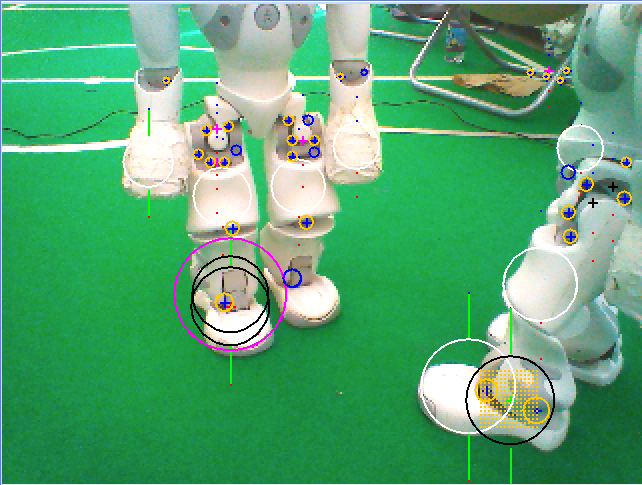
\includegraphics[scale=0.5]{s4.png}
\caption{A record-breaking 25 black spots found in the joints of fellow robots.}
\end{figure}

\begin{figure}[h]
\centering
\label{fig:logs}
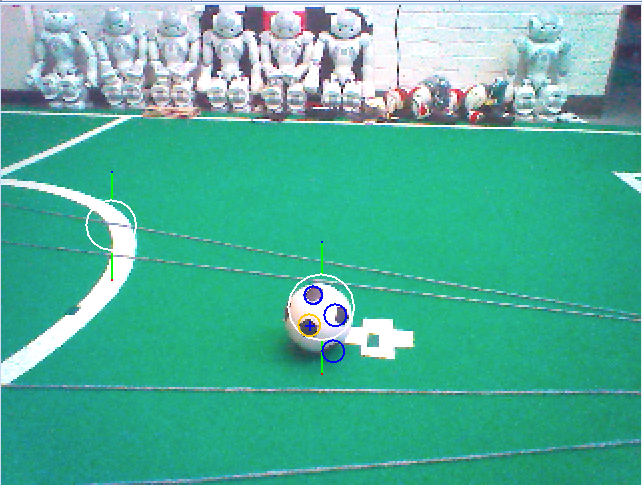
\includegraphics[scale=0.3]{s1.png} \\
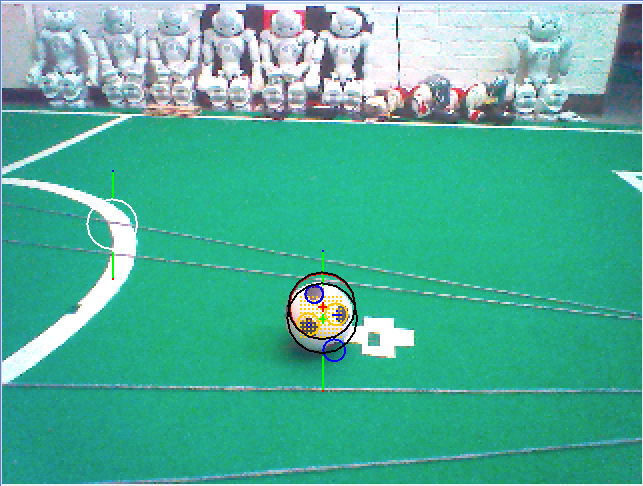
\includegraphics[scale=0.3]{s2.png} \\
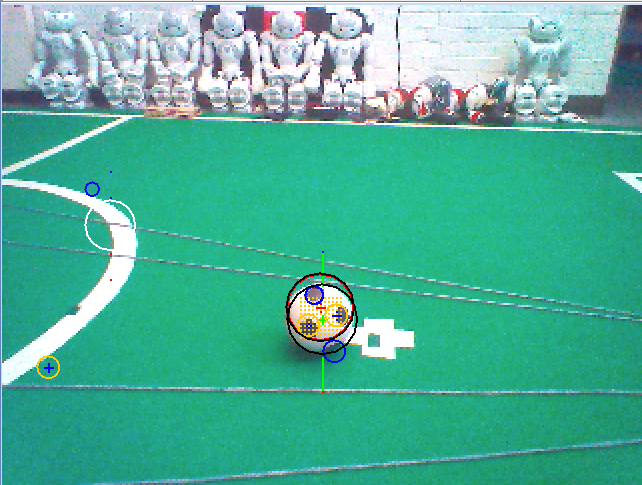
\includegraphics[scale=0.3]{s3.png}
\caption{Three logs taken in the same scenario under lighting conditions of 150 lux. The blue crosses inscribed by yellow circles indicate identified black spots. The red circle (barely visible) in the bottom two images marks a positively identified ball. Note the marked difference in outputs from the ball detector among the three images.}
\end{figure}
\pagebreak
\VerbatimInput{code.cpp}
\end{document}